\documentclass[10pt,a4paper]{article}
%-------------------------------------------
%---Packages--------------------------------
%-------------------------------------------
\usepackage[utf8]{inputenc}
%\usepackage[T1]{fontenc}
%\usepackage{txfonts}
\usepackage{amsmath}
\usepackage{amsthm}
\usepackage{amsfonts}
\usepackage{array}
\usepackage{amssymb}
\usepackage{blindtext}
\usepackage{caption}
\usepackage{color}
\usepackage{csquotes}	    %
\usepackage{enumitem}	    %pour mieux bosser avec les listes. ajoute option label
\usepackage[yyyymmdd]{datetime}        %pour définir date custom
\usepackage{etaremune}
\usepackage{environ}
\usepackage{fancybox}
\usepackage{fancyhdr} 	    % Custom headers and footers
\usepackage{fancyref}
%\usepackage{float}
\usepackage{floatrow}       %float and floatrow can't be together...
\usepackage{gensymb}
\usepackage{graphicx}
\usepackage[colorlinks=true, linkcolor=purple, citecolor=cyan]{hyperref}
\usepackage{footnotebackref}
\usepackage{lipsum}
\usepackage{mathtools}
\usepackage{multicol}	    %gérer plusieurs colonnes
\usepackage{setspace}
\usepackage{subcaption}
\usepackage{todonotes}	    %Bonne gestion des TODOs
%TODO commenté pour tester l'utilité... à voir% \usepackage[tc]{titlepic}      %Permet de mettre une image en page de garde
\usepackage{tikz}	    % Pour outil de dessin puissant
\usepackage{ulem}	    %underline sur plusieurs lignes (avec \uline{})
\usepackage{vmargin} 	    %gestion des marges, avec dans l'ordre : gauche, haut, droit, bas, en-tête, entre en-tête et texte, bas de page, hauteur entre bas de page et texte
\usepackage{wrapfig}
\usepackage{xcolor}
\usepackage{xparse}                    %Pour utiliser NewDocumentCommand et des arguments 'mmooo'
%\usepackage{fullpage} 	    %supprime toutes les marges allouées aux notes, aussi en haut et en bas

%\ExplSyntaxOn
\pagestyle{fancyplain}	    %Makes all pages in the document conform to the custom headers and footers

%-------------------------------------------
%---Document Commands-----------------------
%---------------------------{----------------
\NewDocumentCommand{\framecolorbox}{oommm}
 {% #1 = width (optional)
  % #2 = inner alignment (optional)
  % #3 = frame color
  % #4 = background color
  % #5 = text
  \IfValueTF{#1}%
   {\IfValueTF{#2}%
    {\fcolorbox{#3}{#4}{\makebox[#1][#2]{#5}}}%
    {\fcolorbox{#3}{#4}{\makebox[#1]{#5}}}%
   }%
   {\fcolorbox{#3}{#4}{#5}}%
 }%
%------------------------------------------------
%------------------ENGLISH----------------------
%----------------------------------------------

\NewDocumentCommand{\epflTitle}{mO{Olivier Cloux}O{\today}O{Notes de Cours en}D<>{../../Common}}%Arguments : Matière, Auteur, Date, Titre du doc
{
\begin{titlepage}
    \vspace*{\fill}
    \begin{center}
        \normalfont \normalsize
        \textsc{Ecole Polytechnique Fédérale de Lausanne} \\ [25pt] % Your university, school and/or department name(s)
        \textsc{#4} %Titre du doc
        \\ [0.4 pt]
        \horrule{0.5pt} \\[0.4cm] % Thin top horizontal rule
        \huge #1 \\ % Matière
        \horrule{2pt} \\[0.5cm] % Thick bottom horizontal rule
        
\includegraphics[width=8cm]{#5/EPFL_logo}
        ~\\[0.5 cm]
        \small\textsc{#2}\\[0.4cm]
        \small\textsc{#3}\\
        ~\\
        ~\\
        
\includegraphics[scale=0.5]{#5/creativeCommons}
    \end{center}
    \vspace*{\fill}
\end{titlepage}
}


%-------------------------------------------
%-------------MATH NEW COMMANDS-------------
%-------------------------------------------
\newcommand{\somme}[2]{\ensuremath{\sum\limits_{#2}^{#1}}}
\newcommand{\produit}[2]{\ensuremath{\prod\limits_{#2}^{#1}}}
\newcommand{\limite}{\lim\limits_}
\newcommand{\llimite}[3]{\limite{\substack{#1 \\ #2}}\left(#3\right)}	%limites à deux condiitons
\newcommand{\et}{\mbox{ et }}
\newcommand{\deriv}[1]{\ensuremath{\, \mathrm d #1}}	%sigle dx, dt,dy... des dérivées/intégrales
%\newcommand{\fx}{\ensuremath{f'(\textbf{x}_0 + h}}
\newcommand{\ninf}{\ensuremath{n \to \infty}}	       %pour les limites : n tend vers l'infini
\newcommand{\xinf}{\ensuremath{x \to \infty}}	       %pour les limites : x tend vers l'infini
\newcommand{\infint}{\ensuremath{\int_{-\infty}^{\infty}}}
\newcommand{\xo}{\ensuremath{x \to 0}}									%x to 0
\newcommand{\no}{\ensuremath{n \to 0}}									%n zéro
\newcommand{\xx}{\ensuremath{x \to x}}									%x to x
\newcommand{\Xo}{\ensuremath{x_0}}										%x zéro
\newcommand{\X}{\ensuremath{\mathbf{X}} }
\newcommand{\A}{\ensuremath{\mathbf{A}} }
\newcommand{\R}{\ensuremath{\mathbb{R}} }								%ensemble de R
\newcommand{\rn}{\ensuremath{\mathbb{R}^n} } 							%ensemble de R de taille n
\newcommand{\Rm}{\ensuremath{\mathbb{R}^m} }  							%ensemble de R de taille m
\newcommand{\C}{\ensuremath{\mathbb{C}} }
\newcommand{\N}{\ensuremath{\mathbb{N}} }
\newcommand{\Z}{\ensuremath{\mathbb{Z}} }
\newcommand{\Q}{\ensuremath{\mathbb{Q}} }
\newcommand{\rtor}{\ensuremath{\R \to \R} }
\newcommand{\pour}{\mbox{ pour }}
\newcommand{\coss}[1]{\ensuremath{\cos\(#1\)}}						%cosinus avec des parenthèses de bonne taille (genre frac)
\newcommand{\sinn}[1]{\ensuremath{\sin\(#1\)}}					%sinus avec des parentèses de bonne taille (genre frac)
\newcommand{\txtfrac}[2]{\ensuremath{\frac{\text{#1}}{\text{#2}}}}		%Fractions composées de texte
\newcommand{\evalfrac}[3]{\ensuremath{\left.\frac{#1}{#2}\right|_{#3}}}
\renewcommand{\(}{\left(}												%Parenthèse gauche de taille adaptive
\renewcommand{\)}{\right)}
\newcommand{\longeq}{=\joinrel=}												%Parenthèse droite de taille adaptive


%-------------------------------------------------------
%------------------MISC NEW COMMANDS--------------------
%-------------------------------------------------------
\newcommand{\degre}{\ensuremath{^\circ}}
%\newdateformat{\eudate}{\THEYEAR-\twodigit{\THEMONTH}-\twodigit{\THEDAY}}



%-------------------------------------------------------
%------------------TEXT NEW COMMANDS--------------------
%-------------------------------------------------------
\newcommand{\ts}{\textsuperscript}
\newcommand{\evid}[1]{\textbf{\uline{#1}}}        %mise en évidence (gras + souligné)



%\newcommand{\Exemple}{\underline{Exemple}}
\newcommand{\Theoreme}{\underline{Théorème}}
\newcommand{\Remarque}{\underline{Remarque}}
\newcommand{\Definition}{\underline{Définition} }
\newcommand{\skinf}{\sum^{\infty}_{k=0}}
\newcommand{\combi}[2]{\ensuremath{\begin{pmatrix} #1 \\ #2 \end{pmatrix}}}	%combinaison parmi 1 de 2
\newcommand{\intx}[3]{\ensuremath{\int_{#1}^{#2} #3 \deriv{x}}}				%intégrale dx
\newcommand{\intt}[3]{\ensuremath{\int_{#1}^{#2} #3 \deriv{t}}}				%intégrale dy
\newcommand{\misenforme}{\begin{center} Mis en forme jusqu'ici\\ \line(1,0){400}\\ normalement juste, mais à améliorer depuis ici\end{center}}	%raccourci pour mise en forme
\newcommand*\circled[1]{\tikz[baseline=(char.base)]{
            \node[shape=circle,draw,inner sep=1pt] (char) {#1};}}			%pour entourer un chiffre
\newcommand{\horrule}[1]{\rule{\linewidth}{#1}} 				% Create horizontal rule command with 1 argument of height

\theoremstyle{definition}
\newtheorem{exemp}{Exemple}
\newtheorem{examp}{Example}


%-------------------------------------------
%---Environments----------------------------
%-------------------------------------------
\NewEnviron{boite}[1][0.9]{%
	\begin{center}
		\framecolorbox{red}{white}{%
			\begin{minipage}{#1\textwidth}
 	 			\BODY
			\end{minipage}
		}
	\end{center}
}
\NewEnviron{blackbox}[1][0.9]{%
	\begin{center}
		\framecolorbox{black}{white}{%
			\begin{minipage}{#1\textwidth}
 	 			\BODY
			\end{minipage}
		}
	\end{center}
}
\NewEnviron{exemple}[1][0.8]{%
    \begin{center}
        \framecolorbox{white}{gray!20}{%
            \begin{minipage}{#1\textwidth}
                \begin{exemp}
                    \BODY
                \end{exemp}
            \end{minipage}
        }
    \end{center}
}
\NewEnviron{suiteExemple}[1][0.8]{%
    \begin{center}
        \framecolorbox{white}{gray!20}{%
            \begin{minipage}{#1\textwidth}
                \BODY
            \end{minipage}
        }
    \end{center}
}
\NewEnviron{colExemple}[1][0.8]{%
    \begin{center}
        \framecolorbox{white}{gray!20}{%
            \begin{minipage}{#1\columnwidth}
                \begin{exemp}
                    \BODY
                \end{exemp}
            \end{minipage}
        }
    \end{center}
}
\NewEnviron{example}[1][0.8]{%
    \begin{center}
        \framecolorbox{white}{gray!20}{%
            \begin{minipage}{#1\textwidth}
                \begin{examp}
                    \BODY
                \end{examp}
            \end{minipage}
	}
    \end{center}
}
\NewEnviron{systeq}[1][l]{
			\begin{center}
				$\left\{\begin{array}{#1}
					\BODY
				\end{array}\right.$
			\end{center}
 }





%-------------------------------------------
%---General settings-----------------------
%-------------------------------------------
\renewcommand{\headrulewidth}{1pt}										%ligne au haut de chaque page
\renewcommand{\footrulewidth}{1pt}										%ligne au pied de chaque page
\setstretch{1.6}
\author{Olivier Cloux}

\usepackage{tikz}

\setlength{\leftmargin}{0pt}
\setlength{\rightmargin}{0pt}
\title{Série 4}
\date{}
\author{}
\begin{document}

\maketitle
\evid{Problème 4.1}\\
Notation : \underline{$S^n = (S_1,S_2,S_3,\ldots,s_n)$, P = pile, F = face}
\begin{enumerate}
	\item 	\fbox{$p_{S_0}(A) = 2\cdot\frac{1}{4} = \frac{1}{2}$}\\
			\fbox{$p_{S_0}(B) = p_{S_0}(C) = \frac{1}{4}$}\\
			$H(S_0) = \frac{1}{2}\log_2(2) + \frac{1}{4}\log_2(4)\cdot 2 =$ \fbox{$\frac{3}{2} = H(S_0)$}
	
	\item	Nous devons remarquer 3 cas distincts : \\
			$S^n = (F,F,F,F,F,\ldots,F)\\
			S^n = (P,P,P,P,P,\ldots,P)\\
			S^n = (P,F,P,P,...)$ (tous les autres cas, qui mélangent P et F)
			
			Il y a deux manières d'obtenir le premier cas : tirer la pièce B (donc que des F seront engendrés après), ou tirer une pièce A et tirer, par hasard, que des F. Tirer A et que des F est difficile à avoir : à $n$ tirages, il y a $2^n$ cas (dont un seul nous intéresse), alors que avec B, la probabilité d'avoir F est de 1 (en fait $1^n$ au n\ts{ème} tirage). Nous trouvons donc que $p_{S^n}(FFF...) = \frac{1}{4}\cdot1^n +\frac{1}{2}\frac{1}{2^n} =$\fbox{ $p_{S^n}(FFF...) \frac{1}{4}+\frac{1}{2^{n+1}} = \alpha_n$}\\
			En travaillant un peu $\alpha_n$, nous trouvons\\
			$\alpha_n = \frac{1}{4} + \frac{1}{2^{n+1}} = \frac{2^{n-1}}{2^{n+1}} + \frac{1}{2^{n+1}} = \frac{2^{n-1}+1}{2^{n+1}}$
			
			Le cas \enquote{que des P} est le même que le premier cas (à la différence que l'on souhaite tirer la pièce C ou une A et que des P). La probabilité ne change pas, et \fbox{nous obtenons donc aussi $\alpha_n$ pour $p_{S^n}(PPP...)$}.
			
			Quant aux autres cas, la seule possibilité est de tirer une pièce A et d'ensuite tirer la séquence exacte. Donc \fbox{$p_{S^n}$(reste)$ = \frac{1}{2}\frac{1}{2^n} = \frac{1}{2^{n+1}} = \alpha_n - \frac{1}{4} = \beta_n$}
			
	\item 	Notre source $S^n$ produit une suite de n symboles venant chacun de l'alphabet $D = \{P,F\}$. L'alphabet de $S^n$ est $D^n$. Selon la définition, cette source est donc un \underline{bloc}. Et, comme nous ne précisons pas le nombre de tirages de la pièce (mais nous le supposons très grand, voire infini), le bloc est infini, donc la source est une \evid{Source étendue} \#
	
	\item	Une source est stationnaire si chaque bloc possible a la même probabilité d'apparition. Comme nous venons de le voir, deux blocs - par exemple (FFFFFF....) et (PFPFPFPF....) - n'ont pas du tout la même probabilité d'apparition. Notre source, donc, \underline{n'est pas stationnaire}.
	
	\item	A $n$ tirs, il y a $2^n$ issues possibles :		
			\begin{itemize}
				\item 2 cas (que P ou que F) à probabilité $\alpha_n$.
				\item $2^n-2$ cas (les autres) à probabilité $\frac{1}{2^{n+1}}$
			\end{itemize}
			L'entropie est donc :\\
			$\begin{array}{ll}
				H(S^n) 	& = \alpha_n\log_2(\frac{1}{\alpha_n})\cdot 2 + \frac{1}{2^{n+1}}\log_2(2^{n+1})\cdot(2^n-2)\\
						& = 2\alpha_n\log_2(\frac{1}{\alpha_n}) + \frac{(n+1)(2^n-2)}{2^{n+1}}\\
						& = 2\alpha_n\log_2(\frac{1}{\alpha_n}) + (n+1)\frac{2^n-2}{2^{n+1}}\\
						& = 2\alpha_n\log_2(\frac{1}{\alpha_n}) + (n+1)(\frac{2^n}{2^{n+1}} - \frac{2}{2^{n+1}})\\
						& = 2\alpha_n\log_2(\frac{1}{\alpha_n}) + (n+1)(\frac{1}{2} - \frac{1}{2^n})\\
						& = $\fbox{$2\alpha_n\log_2(\frac{1}{\alpha_n}) + \frac{n+1}{2} - \frac{n+1}{2^n} = H(S^n)$ =  entropie d'un symbole}$
			\end{array}$
			
	\item 	Nous savons que $H(S_b|S_a) = H(S_a,S_b) - H(S_a)$. Si nous posons ensuite $S_n = S_b$ et $S^{n-1} = S_a$, nous pouvons poser :\\
			$H(S_n|S_1,S_2,...,S_{n-1}) = H(S_1,S_2...,S_{n-1},S_n) - H(S_1,...,S_{n-2},S_{n-1})$\\
			Calculer $H(S_n|S^{n-1})$ devient alors plus facile, car nous connaissons $H(S^n)$, et par extension $H(S^{n-1})$ (en remplaçant $n$ par $n-1$ dans notre calcul de l'entropie, précédemment)
			
			Ainsi\\
			$\begin{array}{ll}
				H(S_n|S^{n-1}) 	& = H(S^n) - H(S^{n-1})\\
								& = 2\alpha_n\log_2(\frac{1}{\alpha_n}) + \frac{n+1}{2} - \frac{n+1}{2^n} -\Big( 2\alpha_{n-1}\log_2(\frac{1}{\alpha_{n-1}}) + \frac{(n-1)+1}{2} - \frac{(n-1)+1}{2^{n-1}} \Big)\\
								& = 2\big(\alpha_n\log_2(\frac{1}{\alpha_n})-\alpha_{n-1}\log_2(\frac{1}{\alpha_{n-1}})\big) + \frac{n+1}{2} - \frac{n}{2} -\frac{n+1}{2^n} + \frac{n}{2^{n-1}}\\
								& = 2\big(\alpha_n\log_2(\frac{1}{\alpha_n})-\alpha_{n-1}\log_2(\frac{1}{\alpha_{n-1}})\big) + \frac{1}{2} - \frac{n+1}{2^n} + \frac{2n}{2^{n}}\\
								& = 2\big(\alpha_n\log_2(\frac{1}{\alpha_n})-\alpha_{n-1}\log_2(\frac{1}{\alpha_{n-1}})\big) + \frac{1}{2} + \frac{n-1}{2^n}
			\end{array}$
			Depuis là, nous pouvons commencer à analyser les  cas numériques :
			\begin{itemize}
				\item[n=10] $\alpha_n = \frac{2^9 +1}{2^{11}},\quad \alpha_{n-1} = \frac{2^8+1}{2^{10}}$\\
							$\to H(S_n|S^{n-1}) = 2\big(\frac{2^9+1}{2^{11}}\log_2(\frac{2^{11}}{2^9+1}) - \frac{2^8+1}{2^{10}}\log_2(\frac{2^{10}}{2^8+1})\big) + \frac{1}{2} + \frac{10-1}{2^{10}}$\\
							=\fbox{$ 0.50824$}
				\item[n=15] $\alpha_n = \frac{2^{14} +1}{2^{16}},\quad \alpha_{n-1} = \frac{2^{13}+1}{2^{15}}$\\
							$\to H(S_n|S^{n-1}) = 2\big(\frac{2^{14}+1}{2^{16}}\log_2(\frac{2^{16}}{2^{14}+1}) - \frac{2^{13}+1}{2^{15}}\log_2(\frac{2^{15}}{2^{13}+1})\big) + \frac{1}{2} + \frac{15-1}{2^{15}}$\\
							=\fbox{$ 0.50041$}
				\item[n=20] $\alpha_n = \frac{2^{19} +1}{2^{21}},\quad \alpha_{n-1} = \frac{2^{18}+1}{2^{20}}$\\
							$\to H(S_n|S^{n-1}) = 2\big(\frac{2^{19}+1}{2^{21}}\log_2(\frac{2^{21}}{2^{19}+1}) - \frac{2^{18}+1}{2^{20}}\log_2(\frac{2^{20}}{2^{18}+1})\big) + \frac{1}{2} + \frac{20-1}{2^{20}}$\\
							=\fbox{$ 0.50002$}	
			\end{itemize}

	\item	Rappelons, pour les ingénus qui auraient oublié une telle définition, ce qu'est une source régulière : \\
			\textbf{Une source étendue S est dite \textit{régulière} si les deux limites
			\begin{itemize}
				\item $H(S) \overset{\text{def}}{=} \limite{\ninf}H(S^n)$ et
				\item $H^*(S) \overset{\text{def}}{=} \limite{\ninf}H(S_n|S^{n-1})$
			\end{itemize}
			existent et sont finies.}
			Nous pouvons donc calculer les limites. Commençons $H(S)$ :\\
			$\begin{array}{ll}
				\limite{\ninf}\alpha_n			& \simeq \limite{\ninf}\frac{2^{n-1}}{2^{n+1}} = \frac{1}{4}\\
				\limite{\ninf}\alpha_{n-1}		& = \limite{\ninf}\alpha_n = \frac{1}{4}\\
				\limite{\ninf}\frac{n+1}{2^n}	& \simeq \limite{\ninf}\frac{n}{2^n} = 0\\
				\limite{\ninf}\log_2(\frac{1}{\alpha_n}) & = \log_2(\limite{\ninf}\frac{1}{\alpha_n}) = \log_2(4) = 2\\
			\text{mais :}\\
				\limite{\ninf} \frac{n+1}{2} 	& = \infty
			\end{array}$
			Donc $\limite{\ninf} H(S^n) = \infty$. Donc la source ne peut pas être régulière, car H(S) n'existe pas.
			Calculons quand même l'entropie par symbole :\\
			Nous pouvons reprendre les valeurs des limites calculées précédemment. Cela nous donne donc :\\
			$\begin{array}{ll}\limite{\ninf}H(S_n|S^{n-1}) &= \limite{\ninf} 2\big(\alpha_n\log_2(\frac{1}{\alpha_n})-\alpha_{n-1}\log_2(\frac{1}{\alpha_{n-1}})\big) + \frac{1}{2} + \frac{n-1}{2^n} \\
					&= 2\big(\frac{1}{4}\log_2(4) - \frac{1}{4}\log_2(4)\big) + \frac{1}{2} + 0 \\
					&= 2\cdot(0) + \frac{1}{2} =$ \fbox{$\frac{1}{2}$} $\end{array}$
			
	\item Calculons cette limite :\\
		$\begin{array}{ll}
			\limite{\ninf} \frac{H(S^n)}{n} &= \limite{\ninf}\frac{2\alpha_n\log_2(\frac{1}{\alpha_n}) + \frac{n+1}{2} - \frac{n+1}{2^n}}{n}\\
											&=\frac{\limite{\ninf} 2\alpha_n\log_2(\frac{1}{\alpha_n}) + \frac{n+1}{2} - \frac{n+1}{2^n}}{\limite{\ninf}}\\
											&= \limite{\ninf}\frac{2\alpha_n\log_2(\frac{1}{\alpha_n}) - \frac{n+1}{2^n}}{n} + \limite{\ninf}\frac{\frac{n+1}{2}}{n}\\
											& =  \text{c.f. plus haut } \text{\enquote{$\frac{2\frac{1}{4}\log_2(4) - 0}{\infty}$}} + \limite{\ninf} \frac{n+1}{2n}\\
											&= 0 + \frac{1}{2}\\
											&= $\fbox{$\frac{1}{2}$}$
		\end{array}$
		Nous remarquons que cette limite est la même que $H^*(S)$. En effet, $H^*(S)$ nous dira combien de d'information supplémentaire apportera le dernier tirage, en connaissant les précédents. La limite que nous venons de calculer nous donne le nombre de bits pour un tirage supplémentaire (entropie totale divisée par le nombre de tirages). Cela signifie que l'entropie supplémentaire d'un tirage connaissant les précédents est la même que l'entropie de chaque tirage (à l'infini). De plus, nous savons par le théorème 5.2 que cette égalité doit être respectée.
			
\end{enumerate}

\evid{Problème 4.2}
\begin{enumerate}
	\item	\begin{itemize}
				\item Probabilité de $PP$ et de $FF$ : $\frac{1}{4} + \frac{1}{2}\frac{1}{2^2} = \frac{3}{8}$
				\item Probabilité de $PF$ et de $FP$ : $\frac{1}{2}\frac{1}{2^2} = \frac{1}{8}$
			\end{itemize}
			\begin{multicols}{2}
				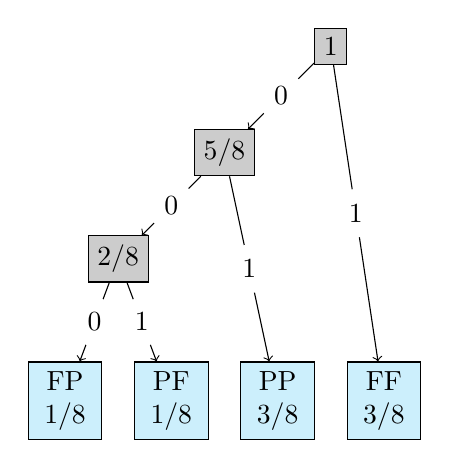
\begin{tikzpicture}[scale=0.9]
					\tikzstyle{etiquette}=[midway, circle ,fill=white]
					\node[draw, fill=black!20] (D) at (-2.25,-1){1};
					\node[draw, text width=0.7cm, text centered, fill = cyan!20] (1) at (-1.5,-6){FF \\ 3/8};
					\node[draw, fill=black!20] (0) at (-3.75,-2.5){5/8};
					\node[draw, text width=0.7cm, text centered, fill = cyan!20] (01) at (-3,-6){PP \\ 3/8};
					\node[draw, fill=black!20] (00) at (-5.25,-4){2/8};
					\node[draw, text width=0.7cm, text centered, fill = cyan!20] (001) at (-4.5,-6){PF \\ 1/8};						
					\node[draw, text width=0.7cm, text centered, fill = cyan!20] (000) at (-6,-6){FP \\ 1/8};

					\draw[->] (D) -- (1)node[etiquette]{1};
					\draw[->] (D) -- (0)node[etiquette]{0};
					\draw[->] (0) -- (00)node[etiquette]{0};
					\draw[->] (0) -- (01)node[etiquette]{1};
					\draw[->] (00) -- (001)node[etiquette]{1};
					\draw[->] (00) -- (000)node[etiquette]{0};
				\end{tikzpicture} \\
				\columnbreak
\\
\\
\\

				\begin{tabular}{r|c|c|c|c}
					Symbole de source & PF & FP & PP & FF \\
					\hline
					Probabilité& $\frac{1}{8}$ & $\frac{1}{8}$ & $\frac{3}{8}$ & $\frac{3}{8}$\\
					\hline
					$\Gamma_{H2}$& 000 & 001 & 01 & 1
				\end{tabular}
			\end{multicols}
			$ L(\Gamma_{H2}) = 2\cdot\frac{1}{8}3 + \frac{3}{8}(1+2)= \frac{20}{8} =$ \fbox{$1.875 =L(\Gamma_{H2})$}\\
			$H(S^2) = 2\cdot\frac{1}{8}\log_2(8) + 2\cdot\frac{3}{8}\log_2(\frac{8}{3}) =$ \fbox{$1.811 = H(S^2)$}\\
			Comme nous nous y attendions, la longueur moyenne du code de Huffman est plus longue que l'entropie. De plus, nous pouvons voir que $\frac{L(\Gamma_{H2}}{2} = \frac{1.875}{2} = 0.9375 >  = H^*(S)$. En effet, $H^*(S)$ est un encodage par blocs, ce qui le rend plus efficace
		
	\item 		\begin{itemize}
				\item Probabilité de $PPP$ et de $FFF$ : $\frac{1}{4} + \frac{1}{2}\frac{1}{2^4} = \frac{5}{16}$
				\item Probabilité de $PPF,\ PFF,\ FFP,\ PFP,\ FPF,\ FPP$  : $\frac{1}{2}\frac{1}{2^3} = \frac{1}{16}$
			\end{itemize}
				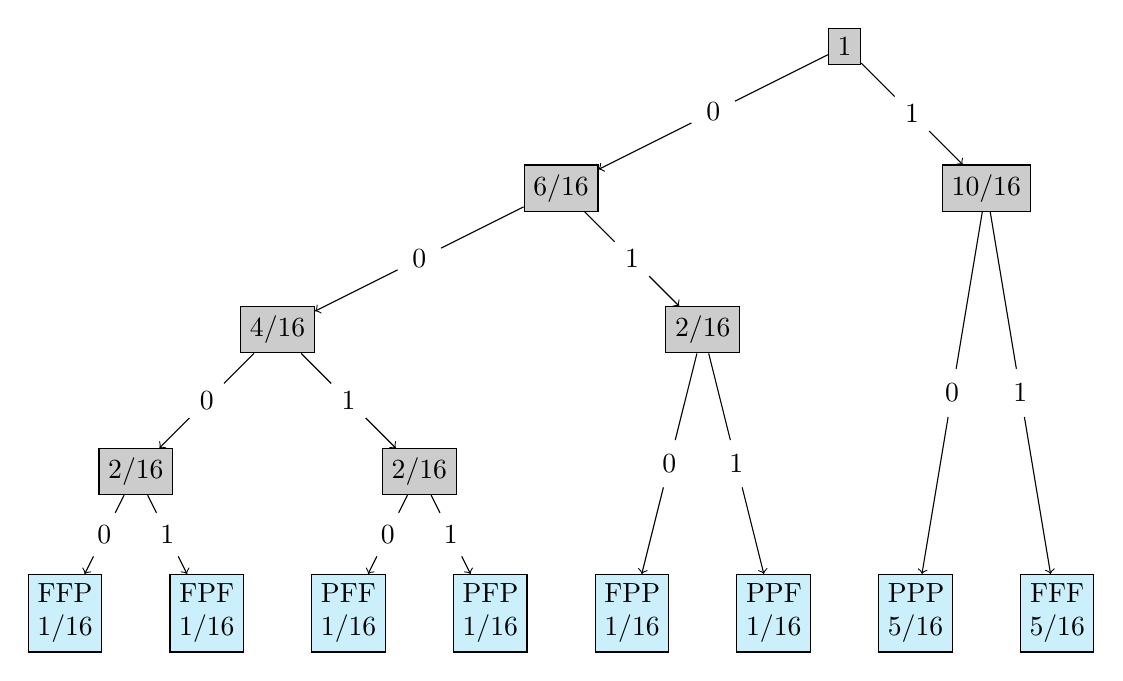
\begin{tikzpicture}[scale=0.9]
					\tikzstyle{etiquette}=[midway, circle ,fill=white]
					\node[draw, fill=black!20] (D) at (0,0){1};
					\node[draw, fill=black!20] (1) at (2, -2){10/16};
					\node[draw, fill=black!20] (0) at (-4,-2){6/16};
					\node[draw, fill=black!20] (01) at (-2, -4){2/16};
					\node[draw, fill=black!20] (001) at (-6, -6){2/16};
					\node[draw, fill=black!20] (000) at (-10, -6){2/16};
					\node[draw, fill=black!20] (00) at (-8, -4){4/16};
					\node[draw, text width=0.7cm, text centered, fill = cyan!20] (10) at (1,-8){PPP \ 5/16};
					\node[draw, text width=0.7cm, text centered, fill = cyan!20] (11) at (3,-8){FFF \ 5/16};
					\node[draw, text width=0.7cm, text centered, fill = cyan!20] (011) at (-1,-8){PPF \ 1/16};
					\node[draw, text width=0.7cm, text centered, fill = cyan!20] (010) at (-3,-8){FPP \ 1/16};
					\node[draw, text width=0.7cm, text centered, fill = cyan!20] (0011) at (-5,-8){PFP \ 1/16};
					\node[draw, text width=0.7cm, text centered, fill = cyan!20] (0010) at (-7,-8){PFF \ 1/16};
					\node[draw, text width=0.7cm, text centered, fill = cyan!20] (0001) at (-9,-8){FPF \ 1/16};
					\node[draw, text width=0.7cm, text centered, fill = cyan!20] (0000) at (-11,-8){FFP \ 1/16};

					\draw[->] (D) -- (1)node[etiquette]{1};
					\draw[->] (D) -- (0)node[etiquette]{0};
					\draw[->] (0) -- (00)node[etiquette]{0};
					\draw[->] (0) -- (01)node[etiquette]{1};
					\draw[->] (1) -- (11)node[etiquette]{1};
					\draw[->] (1) -- (10)node[etiquette]{0};
					\draw[->] (01) -- (011)node[etiquette]{1};
					\draw[->] (01) -- (010)node[etiquette]{0};
					\draw[->] (001) -- (0011)node[etiquette]{1};
					\draw[->] (001) -- (0010)node[etiquette]{0};
					\draw[->] (00) -- (001)node[etiquette]{1};
					\draw[->] (00) -- (000)node[etiquette]{0};
					\draw[->] (000) -- (0001)node[etiquette]{1};
					\draw[->] (000) -- (0000)node[etiquette]{0};
				\end{tikzpicture} \\
				\begin{tabular}{r|c|c|c|c|c|c|c|c}
					Symbole de source & FFP & FPF & PFF & PFP & FPP & PPF & PPP & FFF \\
					\hline
					Probabilité& $\frac{1}{16}$ & $\frac{1}{16}$ & $\frac{1}{16}$ & $\frac{1}{16}$ & $\frac{1}{16}$ & $\frac{1}{16}$ & $\frac{5}{16}$ & $\frac{5}{16}$\\
					\hline
					$\Gamma_{H3}$& 0000 & 0001 & 0010 & 0011 & 010 & 011 & 10 & 11\\
				\end{tabular}\\
				$L(\Gamma_{H3}) = 4\frac{1}{16}\times4  + 3\frac{1}{16}\times2 + 2\frac{5}{16}\times2 =$ \fbox{$2.625 = L(\Gamma_{H3})$}\\
				$H(S^3) = \frac{1}{16}\log_2(16)\times 6 + \frac{5}{16}\log_2(\frac{16}{5}) \times 2 = $\fbox{$2.5488 =H(S^3)$}\\
				La différence entre $L(\Gamma_{H3})$ et $H(S^3)$, avec l'entropie plus faible que la longueur moyenne, n'est pas surprenante (cf les 3 séries précédentes : \enquote{on ne peut pas faire mieux que l'entropie})\\
				Cependant, $\frac{L(\Gamma_{H3})}{3} = \frac{2.625}{3} = 0.875 > 0.5 = H^*(S)$. En effet, $H^*(S)$ est un encodage par blocs, ce qui le rend plus efficace. Finalement, nous pouvons remarquer que, par rapport à $\Gamma_{H3}$, la longueur moyenne par bloc semble se rapprocher de $H^*(S)$ ; 
	\item 	Comme nous l'avons montré et calculé précédemment, au 1000\ts{ème} tirage, 2 résultats ($PPP\ldots PP$ et $FFF\ldots FF$) auront une probabilité de\\
			$\frac{1}{4}+\frac{1}{2^{1001}} = \frac{2^{999}+1}{2^{1001}} 0.25000000000000000000000000000000000000000000000000000000000000000000000\\
			000000000000000000000000000000000000000000000000000000000000000000000000000000000\\
			00000000000000000000000000000000000000000000000000000000000000000000000000000\\
			00000000000000000000000000000000000000000000000000000000000000000000000046663\\
			18092516094394950447723619085848085457231858540123108571698979834554878878172$ (donc environ 0.25)

			Les $ 2^{1000}-2$ autres auront une probabilité de $\frac{1}{2^{1001}}$ (vous l'aurez compris, c'est très petit, je ne vais pas mettre le chiffre exact ici ;-) )\\
			Il s'agit ensuite d'utiliser l'algorithme de Shannon pour cela : rappelons-nous que la longueur des mots de code, selon Shannon-Fano, est de $\lceil\log_2(\frac{1}{p_i})\rceil$\\
			Pour cette majorité d'outcomes, chacun aura une longueur de mots de\\
			$\lceil\log_2(2^{1001})\rceil = \lceil1001\rceil = 1001$\\
			Pour les deux autres (uniquement pile et ou face), ils auront une longueur de\\
			$\lceil\log_2(\frac{2^{1001}}{2^{999}+1})\rceil = \lceil 1.999[...]730 \rceil = 2$ ([...] représente une grande quantité (finie) de \enquote{9})\\
			Cela nous donne une longueur moyenne de\\
			$L(\Gamma_{SF}) =1001\frac{1}{2^{1001}}\times(2^{1000}-2) +  2(\frac{1}{4}+\frac{1}{2^{1001}})\times 2 \simeq 501.500000$\\
			$H(S^{1000}) = 2 \frac{2^{999} + 1}{2^{1001}}\log_2(\frac{2^{1001}}{2^{999}+1}) + \frac{1000 + 1}{2} - \frac{1000 + 1}{2^{1000}} \simeq 501.500000$\\
			\\
			Longueur moyenne par symbole = $\frac{501.500000}{1000}	= 0.5015 > 0.5 = H^*(S) =$ entropie par symbole.\\
			Avec un nombre de tirages très grand, la probabilité de \enquote{que pile} et de \enquote{que face} tend vers 1/4 (donc tirer une pièce truquée, car tirer 1000x de suite la même chose avec une pièce pas truquée est extrêmement faible), donc \enquote{que pile ou que face} tend vers $1/2$. De plus, l'entropie de Shannon va tendre vers $n/2$. Si nous cherchons la longueur moyenne par symbole, nous divisons encore cela par $n$, donc vers $\frac{1/2 + n/2}{n}$, donc vers $\frac{1}{2}$. A l'infini, tend donc vers l'efficacité de l'entropie.

	\item	Pour les $2^{1000}-2$ cas banals, nous avons vu qu'ils auront une longueur encodée de 1001 bits. Avec $1000$ lancés, le bloc($S_1,S_2,...,S_{1000}$) est de longueur 1000. Il suffit donc de changer chaque résultat de chaque lancé en un chiffre (par exemple Pile devient 1, Face devient 0), et d'ajouter un 0 avant (pour respecter la longueur de Shannon, et éviter les préfixes avec les 2 cas particuliers). De cette manière, comme chaque bloc ($S_1,...,S_{1000}$) est unique, son encodage le sera aussi.\\
			Les deux cas particuliers seront juste encodés sur 2 bits : le premier serait 1(pour éviter les préfixes avec les cas banals), et le second serait 1 pour Pile et 0 pour Face. \\
			\\
			La longueur moyenne de notre code est de 501.5. Transformer chaque tirage en 1 ou 0 selon la méthode proposée donnerait un code de longueur 1000. Le rapport de compression est donc $\frac{501.5}{1000} = 0.5015$, ce qui est notre rapport de compression. Notre méthode de codage nous permet donc de compresser considérablement le code.

\end{enumerate}
\end{document}